\Section
{پیش‌پرداز‌ش‌های انجام‌شده}
{
	\subsection{روش/ابزار تفکیک جملات}
	{
		بری تفکیک جملات از ابزار
		\lr{nltk}
		که یک ابزار معروف در حوزه
		\lr{NLP}
		می باشد استفاده کردم. این ابزار یک تابع 
		\lr{sent\_tokenize}
		دارد که یک عبارت می گیرد و در خروجی یک لیست از جملاتی که در آن عبارت وجود دارد برمی گرداند.
	}
	\subsection{روش/ابزار تفکیک توکن‌ها/کلمات}
	{
		برای جدا کردن کلمات از 
		\lr{إBERT Tokenizer}
		استفاده کردم.
		\lr{BERT}
		یک مدل زبانی 
		\lr{transformer-based}
		می باشد که به صورت گسترده برای تولید
		\lr{embedding}
		کلمات به کار می رود. من در این پروژه از این 
		\lr{tokenizer}
		استفاده کردم و ابتدا هر جمله را 
		\lr{encode}
		کردم و به
		\lr{input\_ids}
		تبدیل کردم و  سپس با تابع 
		\lr{convert\_ids\_to\_tokens}
		آنها را تبدیل به توکن/کلمه کردم و ذخیره کردم
		\\ لازم به دکر است که چون تعداد توییت ها بالا است برای جلوگیری از زمان بر بودن این فرایند از 
		\lr{BertTokenizerFast}
		استفاده کردم که پیاده سازی آن با زبان 
		\lr{Rust}
		بوده و بسیار سریع تر عمل می کند.
	}
	
	\subsection{روش/معیارهای تمیزکردن داده}
	{ 
		\subsubsection{\Large حذف کاراکتر های غیر لاتین}
		{
			در بین توییت های موجود در دیتاست برخی به زبان فارسی یا چینی و زبان های مختلفی بودند که مجبور شدیم آنها را حذف کنیم. دلایل این کار عبارتند از:
			\begin{itemize}
				\item 
				حجم عطیمی از دیتاست به زبان انگلیسی است و
				\lr{BERT tokenizer}
				هم با زبان انگلیسی آموزش دیده است در صورتی که کلماتی غیر از کلماتی که در 
				\lr{vocabulary}
				خود وجود دارد ببینید به آنها توکن
				\lr{unknown}
				نسبت می دهد که این کار باعث می شود تا حجم داده غیر مفید بالا برود و بازدهی مدل در هنگام یادکیری پایین بیاید
				%%%%%%%%%%%%
				\item 
				وجود کلمات چینی به دلیل اینکه بیشتر بصری هستند و از این لحاط به هم نزدیکی دارند نیاز دارد تا یک لایه
				\lr{CNN}
				برای در ک بهتر به 
				\lr{tokenizer}
				اضافه شود. ولی خب من ترجیح دادم تا تمام کاراکتر ها به یک زبان باشند تا مدل به راحتی یاد بگیرد و رابطه بین کلمات را بهتر متوجه بشود تا در نهایت یک 
				\lr{embedding}
				بهتر خروجی بدهد
			\end{itemize}
			
		}
		\subsubsection{\Large حذف کلمات پالایشی (\lr{stopwords})}
		{
			منظور از کلمات پالایشی کلماتی مثل 
			\lr{the}
			،
			\lr{and}
			،
			\lr{is}
			،
			\lr{in}
			،
			\lr{it}
			و... است.
			این کلمات دربردارنده بار معنایی ارزشمندی برای تشخیص لحن نیستند و به همین دلیل با حذف آن‌ها از متن ورودی می‌توانیم حجم نویز ورودی را کم کنیم و به مدل اجازه دهیم بتواند روی کلمات کلیدی‌تر متن ورودی تمرکز کند.
			
			برای حذف این کلمات از پکیج \lr{nltk} استفاده شده است.
		}
		\subsubsection{\Large حذف کردن (\lr{mention} ها)}
		{
			در توییت ها زیاد اتفاق می افتد تا در آخر توییت چندین نفر را به صورت "\lr{@username}" منشن کنند.
			این بخش از توییت هیچ ارزش خبری ندارد و داده اضافی و غیر مفید است و باید حذف شود
		}
		\subsubsection{\Large حذف (\lr{urls})}
		{
			در توییت ها ممکن است لینک دسترسی به یک خبر یا چیز های مختلفی برای ارجاع به چیزی داده شود که محتوی خود این 
			\lr{url}
			برای ما ارزشی ندارد و مدل نباید آن را در نظر بگیرد زیرا ممکن است گمراه شود و به اشتباه کاراکتر های موجود در
			\lr{url}
			را مهم تلقی کند. این اطلاعات هم غیر مفید است و باید حذف شود
		}
		\subsubsection{\Large حذف اعداد و علائم نشانه گذاری (\lr{punctations})}
		{
			در توییت ها برای خوانایی بیشتر از علائم نشانه گذاری استفاده می شود که عبارتند از:
			\begin{itemize}
				\item : (\lr{colon})
				\item ; (\lr{semicolon})
				\item ' (\lr{apostrophe})
				\item , (\lr{comma})
				\item {[]} (\lr{square brackets})
				\item () (\lr{parentheses})
			\end{itemize}
			به نظر نمی رسد تاثیری در لحن یک جمله داشته باشد و بهرت است حذف شود
			همچنین ارقام نیر تاثیری در لجن یک توییت ندارند. مثلا این طور نیست که عدد 9 لحن مثبت داشته باشد و عددد 0 لحن منفی داشته باشد و برای جلوگیری از این بدفهمی بهتر است حذف شوند و به آنها توجی نشود.
		}
		\subsubsection{\Large تبدیل کلمات به \lr{lowercase}}
		{
			در آخر کار تمام کلمات را به 
			\lr{lowercase}
			تبدیل کردیم تا مدل راحت تر بتواند یاد بگیرد و به طور مثال فرقی بین 
			\lr{A} و \lr{a}
			نگذارد زیرا در عمل هم فرقی ندارند.
		}
	}
	\newpage
	\subsection{اندازه داده قبل/بعد تمیزکردن داده}
	{
		برای کلمات:
		\begin{center}
			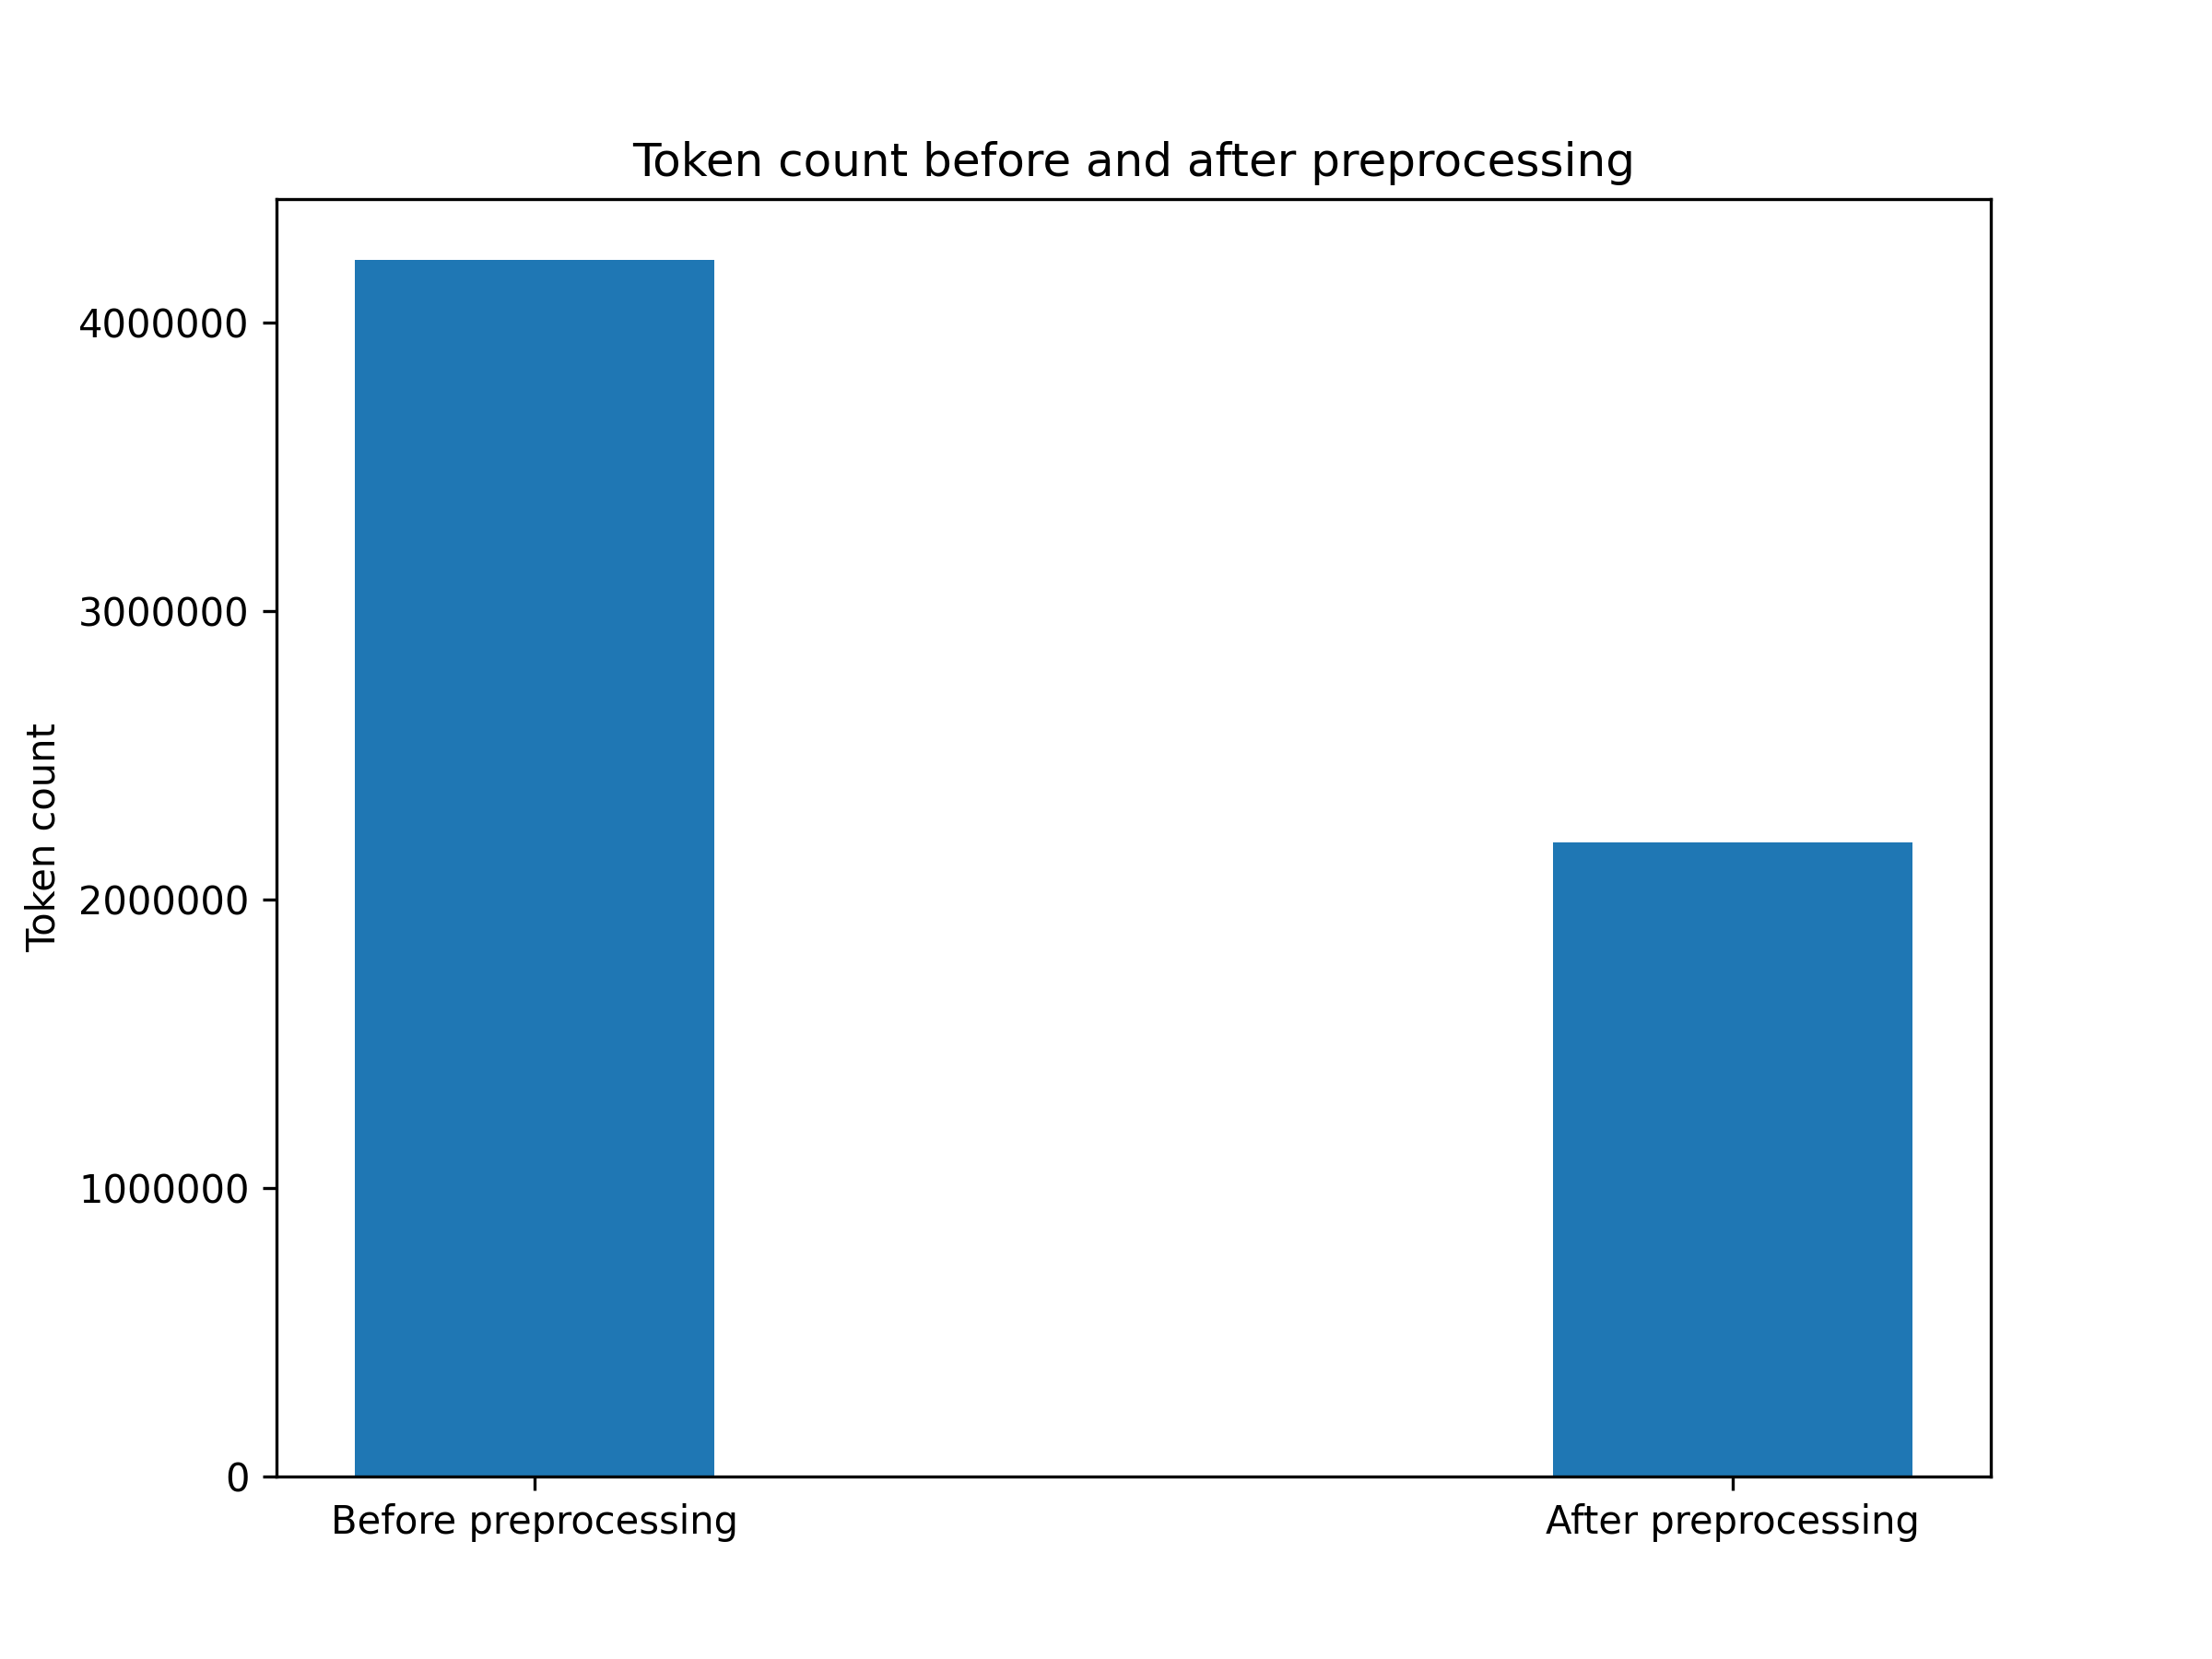
\includegraphics[scale=0.55]{../stats/token_counts_befor_after_pre_processing.png}
		\end{center}
		% \begin{adjustbox}{width=\textwidth}
			% 	\csvautotabular{../stats/token_counts_befor_after_pre_processing.csv}  
			% \end{adjustbox}
		
		
		برای جملات:
		\begin{center}
			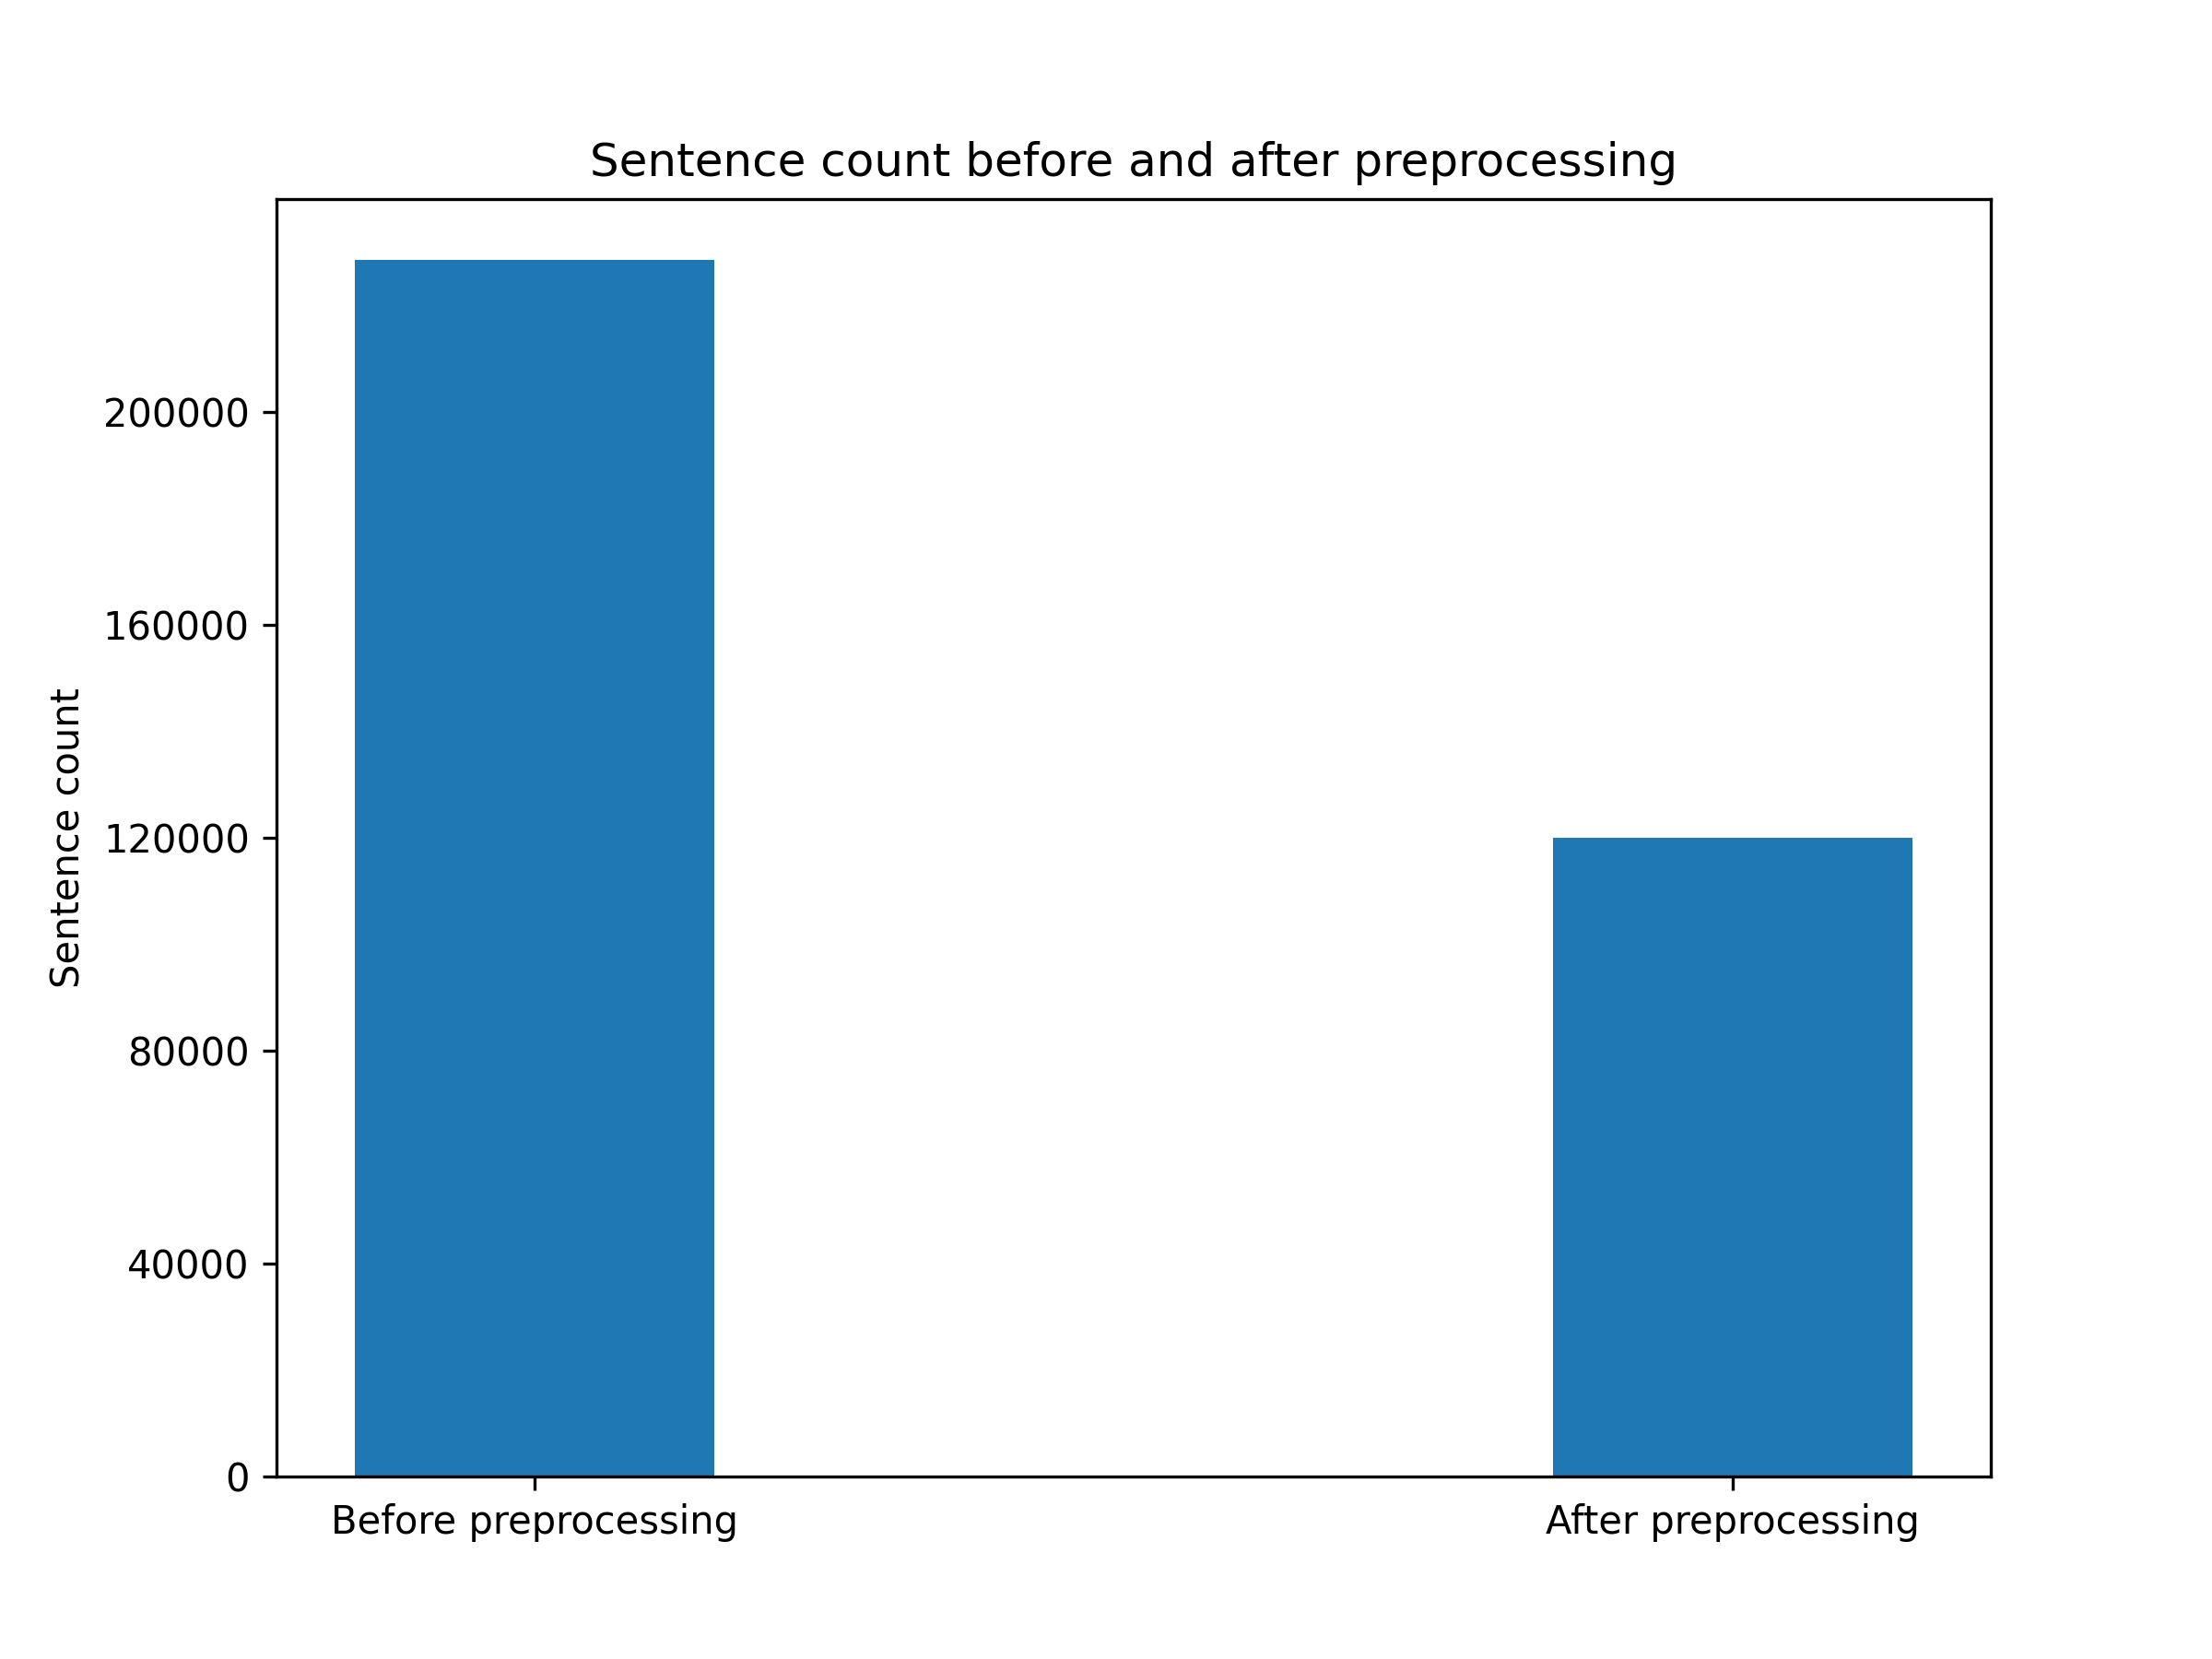
\includegraphics[scale=0.55]{../stats/sentence_counts_befor_after_pre_processing.png}
		\end{center}
		% \begin{adjustbox}{width=\textwidth}
			% 	\csvautotabular{../stats/sentence_counts_befor_after_pre_processing.csv}  
			% \end{adjustbox}
	}
}